\documentclass[12pt,a4paper]{article}
\newcommand{\AuthorName}
{سپهر صفری، سارا خسروی، پرهام صارمی}
\newcommand{\AuthorSTID}
{97108263, 97101586, 97101959}

\usepackage{commons/course}
\usetikzlibrary{automata, positioning, arrows}

\lstset{
numbers=left, 
numberstyle=\small, 
numbersep=8pt, 
frame = single, 
language=Python,
framexleftmargin=15pt
}





%
%\let\ds\displaystyle
%\usepackage{arabtex}
%\usepackage[utf8]{inputenc}
%\usepackage[LFE,LAE]{fontenc}
%\usepackage[english,farsi]{babel}
%


\begin{document}


\سربرگ{پاسخ تمرین سری دوم}{پارسر‌ها}{98/12/25}



%نام و نام خانوادگی:
%شماره دانشجویی:
\مسئله{}

\پاسخ{}
\\
در شکل زیر 
tree activation
را برای کد داده شده مشاهده می‌کنید.
لازم به ذکر است که متغیرهای محلی
در این شکل با رنگ قرمز نشان داده شده‌اند.
ورودی‌های تابع به همان رنگ مشکی می‌باشند.
\begin{figure}[htp]
    \centering
    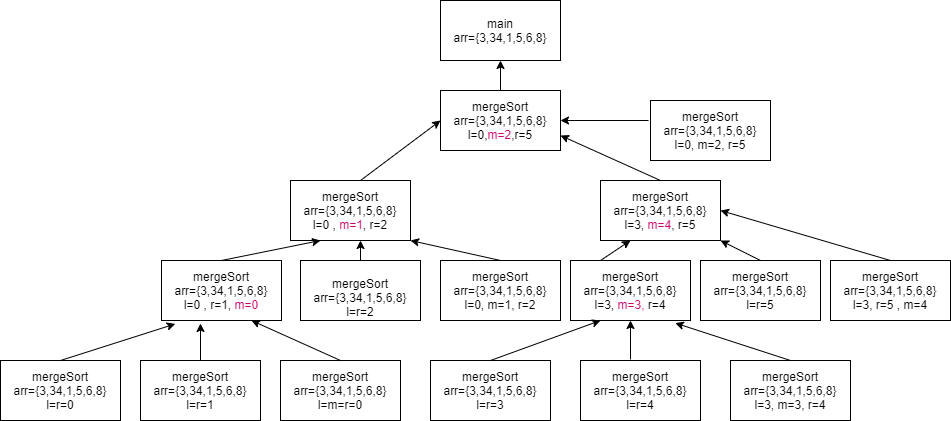
\includegraphics[width=18cm]{q1.png}
    \caption{actication tree}
\end{figure}  

%نام و نام خانوادگی:
%شماره دانشجویی: 
\مسئله{ }

\پاسخ{}
\\

الف)
در ابتدا که مانند تمام حالات دیگر، fp
و ra
را تعین می‌کنیم.
\\
پس از آن با تابع
main
سر و کار داریم که خط به خط اجرا خواهد شد. بخش نخست
frame
stack 
نیز مختص این تابع است.
ابتدا مقادیر دو متغیر محلی 
a
و
b
 در سر استک قرار خواهند گرفت. در این حالت تابع main
 همان تابع caller
 ماست که این مقادیر را push
 می‌کند.
 سپس اجرای برنامه به تابع gcd
 می‌رسد.
 این مقدار نیز توسط تابع main
 مانند مقادیر قبلی در stack
 قرار می‌گیرد.
 \\
 سپس با فراخوانی تابع جدید، از تابع main خارج شده
 و برای نخستین بار با اجرای تابع gcd
 مقادیر را در استک قرار می‌دهیم.
 این بخش ، بخش دوم شکل ماست.
 در این حالت تابع main
 مقادیر x
 و
 y
 و 
 fp
 و
 ra
 را درون استک قرار خواهد داد.
مقادیری که این تابع در نهایت بازخواهد گرداند، توسط خود این تابع 
gcd
درون استک قرار داده خواهد شد. 
یعنی خطوط 8 و 11 توسط تابع gcd
که برای بار نخست صدا زده شده است ، پر می‌شوند.
\\
سپس مشابه بخش دوم، بخش سوم استک را هم پر می‌کنیم.
این بخش مربوط به اجرای تابع 
gcd
برای بار دوم است.
زمانی که برای اولین بار خط 11 ام برنامه اجرا شود،
خانه‌های 6ام به بعد استک نیز شروع به پر شدن می‌کنند.
سپس به جایی میرسیم که شرط اول تابع 
gcd
برقرار است و مجددا مقادیر قابل بازگشت در استک توسط خود تابع
gcd
در استک قرار می‌گیرند. یعنی خانه‌های 14 و 17.
لازم به ذکر است که این مقادیر توسط تابع gcd
نخست push می‌شوند.
\\
سپس تابع برای بار سوم اجرا شده و این را در بخش چهارم استک میبینید.
در این بخش هم 
مشابه بخش قبل مقادیر داخل استک قرار خواهند گرفت با این فرق که این بار تابع
gcd
دوم
این مقادیر را push
می‌کند.
لازم به ذکر است که اگر هر خانه را 4تایی فرض کنیم،
خانه اول اگر آدرسش x
باشد،
خانه‌های 9 ام و 15ام و 21 ام به ترتیب برابر 
x
و
x-28
و
x-48
خواهند شد.
\\
پس همانطور که پیش‌تر گفته شد،
که برای اولین بار خط 11 ام برنامه اجرا شود،
خانه‌های 6ام به بعد استک نیز شروع به پر شدن می‌کنند
\\
ب)
\\
توضیحات مانند قبل است.
با اتمام اجرای خط هشتم،
چون دیگر تابعی صدا زده نمیشود و مرحله به مرحله از هر تابع برمیگردیم تا تا کل استک از بالا به پایین 
رفته و به خط 5 میرسد و متغیر محلی
c
مقدار 12 را به خود می‌گیرد.

\begin{figure}[htp]
    \centering
    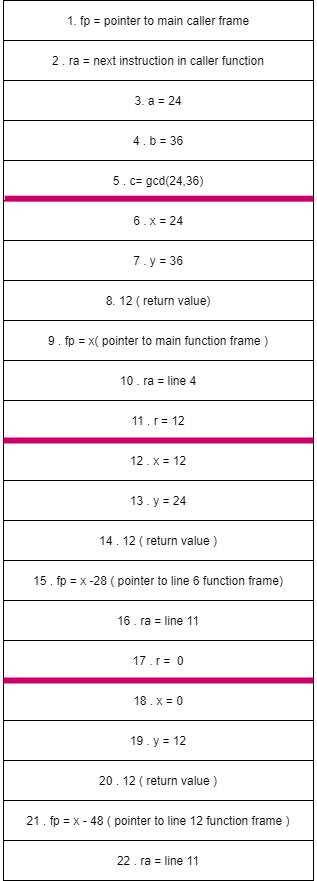
\includegraphics[width=8cm]{images/q2.png}
    \caption{frame Stack }
\end{figure}  

%نام و نام خانوادگی:
%شماره دانشجویی: 
\مسئله{\lr{Recursive Descent}}
\پاسخ{
در این گرامر عبارت E دارد یک جمله شامل جمع و یا تفریق چند عبارت T می‌باشد (یا یک T تنها) بنابراین ابتدا برای حذف \lr{left recursion} گرامر را به صورت زیر تغییر می‌دهیم:
\begin{align*}
	\textcolor{red}{E} \rightarrow \textcolor{red}{T}\textcolor{blue}{+} \textcolor{red}{E}|\textcolor{red}{T}\textcolor{blue}{-}\textcolor{red}{E}|\textcolor{red}{T}
\end{align*}
حال با توجه به اینکه سه عبارت داریم که با T شروع می‌شوند با استفاده از \lr{factoring} گرامر به صورت زیر تبدیل می‌شود:

\begin{align*}
	\textcolor{red}{E} \rightarrow \textcolor{red}{T}\textcolor{red}{E'}\\
	\textcolor{red}{E'} \rightarrow \textcolor{blue}{+}\textcolor{red}{E}|\\
	\textcolor{blue}{-}\textcolor{red}{E}|\\
	\textcolor{blue}{\epsilon}
\end{align*}
حال به رفع مشکل عبارت T می‌پردازیم از آنجایی که نشان دهنده‌ی دنباله‌‌ای از دو عبارت \lr{10} یا \lr{11} می‌باشد،‌ گرامر زیر را جایگزین T می‌کنیم که نشان دهنده‌ی این نوع عبارات می‌باشد:
\begin{align*}
	\textcolor{red}{T} \rightarrow \textcolor{red}{B}\textcolor{red}{T}\\
	\textcolor{red}{B} \rightarrow \textcolor{blue}{1}\textcolor{red}{C}\\
	\textcolor{red}{C} \rightarrow \textcolor{blue}{1}|\textcolor{blue}{0}
\end{align*}
حال الگوریتم به صورت \lr{LL(1)} تبدیل شده است بنابراین شبه‌‌کدهای پایتون زیر را برای این گرامر‌ها استفاده می‌کنیم:
\begin{latin}
	code here
\end{latin} 
}

%نام و نام خانوادگی:
%شماره دانشجویی: 
\مسئله{تبدیل \lr{NFA}  به \lr{DFA} }

\پاسخ{}
\\
1.
\\
در کل m+n+1 استیت در نظر میگیریم. از استیت m به بعد، با اپسیلون تمام حالات موجود را به حالت نهایی برده و اکسپت میکینم،  سپس برای حالاتی هم که از n تا بیشتر بودند، یک استیت دیگر داریم که ازین به بعد تمام حروف الفبایی که میگیریم را در آن استیت میبریم که قابل قبول نباشد.
تا پیش از استیت m را نیز هر 
بار با دریافت هر حرف الفبایی به استیت بعدی میرویم.
استیتهای میانی با ... مشخص شده اند.
\\
\newpage

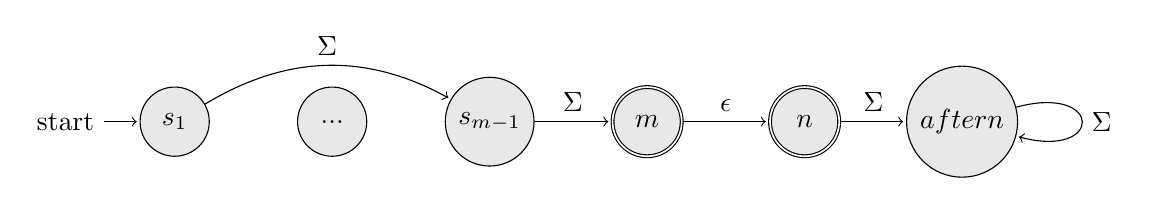
\begin{tikzpicture}[shorten >=1pt,node distance=2cm,on grid,auto]
\tikzstyle{every state}=[fill={rgb:black,1;white,10}]
\node[state,initial]   (s1)                    {$s_1$};
\node[state]   (...)      [right of=s1]               {$...$};
\node[state]  (sm) [right of=...]              {$s_{m-1}$};
\node[state,accepting]   [right of=sm]   (m)                    {$m$};
\node[state,accepting] (n)  [right of=m]    {$n$};
\node[state]           (aftern)  [right of=n]    {$after n$};
\path[->]
(s1) edge [bend left]  node {{$\Sigma$}}    (sm)
(sm) edge []  node {{$\Sigma$}}    (m)
(m) edge []  node {{$\epsilon$}}    (n)
(n) edge []  node {{$\Sigma$}}    (aftern)
(aftern)	edge [loop right] node {{$\Sigma$}}    (   );
\end{tikzpicture}


2.
\\
در کل 6 مسیر aabb را مشخص میکنند:
\\
1223
\\
1100
\\
0111
\\
0110
\\
0112
\\
0122\\
که از بین آنها مسیر زیر 1223 در استیت نهایی رشته را تمام میکند و لذا رشته قابل تشخیص است.
\\
3.
در هر یک از استیتها که باشیم، 2 حالت قابل قبول برای رسیدن به رشته مورد نظر وجود دارد لذا 2 به توان 4 و یا 16 حالت وجود دارد.


\مسئله{}
\پاسخ{}

برای اینکه با sp به مشکل بخوریم باید کد ما در یک تابع شامل \lr{dynamic stack allocation} باشد زیرا اگر چنین چیزی داشته باشیم نمیدانیم برای اینکه به ورودی‌ها دسترسی داشته باشیم باید چند خانه در استک به عقب برگردیم زیرا در زمان اجرا مقداری حافظه به استک اضافه شده که در زمان کامپایل وجود نداشته و ما از این مقدار اطلاعی نداریم بنابراین برای دسترسی به ورودی‌ها مجبوریم از fp استفاده کنیم کد زبان سی به صورت زیر است که آن را به TAC تبدیل می‌کنیم:
\begin{latin}
	\begin{verbatim}
		void allocateStackAndMakeSPUseless(int x, int a){
		    char* mem = _malloca(x);
		    c = 2*a;
		}
	\end{verbatim}
\end{latin}
که کد TAC آن به صورت زیر می‌باشد:
\begin{latin}
	\begin{verbatim}
		allocateStackAndMakeSPUseless:
		    BeginFunc 20;
		    _t0 = x;
		    PushParam _t0;
		    _t1 = LCall _MallocA;
		    PopParams 4;
		    _t2 = 2 * a;
		    EndFunc;
			
	\end{verbatim}
\end{latin}
در این کد فرض شده که \lr{MallocA} در TAC مانند Alloc در اسلاید‌های درس عمل می‌کند

%نام و نام خانوادگی:
%شماره دانشجویی: 
\مسئله{پارسر LR(0)}

\پاسخ{}
\\
\\
الف.
\\
\\
\begin{latin}
\begin{enumerate}
    \item 
    S' -> {$\cdot$} S {$\textdollar$}, S -> {$\cdot$} A , A -> {$\cdot$} a A b , A -> {$\cdot$} a A c, A -> {$\cdot$} d b
    \item
    A -> a {$\cdot$} A b , A -> a {$\cdot$} A c , A -> {$\cdot$} a A b , A -> {$\cdot$} a A c , A -> {$\cdot$} d b
    \item
    A -> d {$\cdot$} b
    \item
    S' -> S {$\cdot$} {$\textdollar$}
    \item
    S -> A {$\cdot$}
    \item
    S' -> S {$\textdollar$} {$\cdot$}
    \item
    A -> d b {$\cdot$}
    \item
    A -> a A {$\cdot$} b , A -> a A {$\cdot$} c
    \item
    A -> a A b {$\cdot$}
    \item
    A -> a A c {$\cdot$}
\end{enumerate}
\end{latin}

\begin{center}
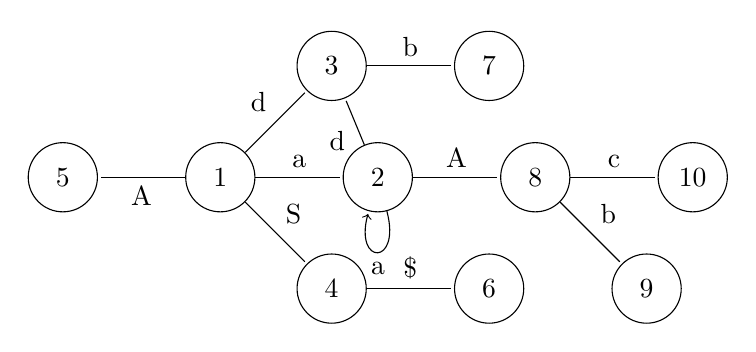
\begin{tikzpicture}[shorten >=1pt,node distance=2cm,on grid,auto]
\node[state]   (R1)                    {$1$};
\node[state]   (R2)       [right of=R1]              {$2$};
\node[state]  (R3)       [above right of=R1]    {$3$};
\node[state]  (R4)        [below right of=R1]        {$4$};
\node[state]  (R5)         [left of=R1]      {$5$};
\node[state]  (R6)        [right of=R4]       {$6$};
\node[state]  (R7)        [right of=R3]  {$7$};
\node[state]  (R8)          [right of=R2]      {$8$};
\node[state]  (R9)       [below right of=R8]       {$9$};
\node[state]  (R10)    [right of=R8]       {$10$};

\path (R1) edge []  node {a}    (R2);
\path (R1) edge []  node {S}    (R4);
\path (R1) edge []  node {d}    (R3);
\path (R1) edge []  node {A}    (R5);
\path (R2) edge []  node {d}    (R3);
\path (R2) edge [loop below]  node {a}    (R2);  
\path (R2) edge []  node {A}    (R8);
\path (R3) edge []  node {b}    (R7);
\path (R4) edge []  node {{$\textdollar$}}    (R6);
\path (R8) edge []  node {c}    (R10);
\path (R8) edge []  node {b}    (R9);
\end{tikzpicture}
\end{center}
ب.
\\
\\
\begin{latin}
\begin{tabular}{ | m{5cm} | m{5cm} | m{5cm} |  } \hline
stack & remaining input & action \\ \hline
S' -> {$\cdot$}S{$\textdollar$} & a a d b c {$\textdollar$} &  \\ 
S -> {$\cdot$} A & & \\ 
A -> {$\cdot$} a A b & & \\
A -> {$\cdot$} a A c & & \\
A -> {$\cdot$} d b & & \\ \hline

S' -> {$\cdot$}S{$\textdollar$} & a d b c {$\textdollar$} & shift  \\ 
S -> {$\cdot$} A & & \\ 
A -> {$\cdot$} a A b & & \\
A -> {$\cdot$} a A c & & \\
A -> {$\cdot$} d b & & \\
A -> a {$\cdot$} A b & &\\ 
A -> a {$\cdot$} A c & & \\ 
A -> {$\cdot$} a A b & & \\
A -> {$\cdot$} a A c & & \\
A -> {$\cdot$} d b & & \\ \hline

S' -> {$\cdot$}S{$\textdollar$} & d b c {$\textdollar$} & shift  \\ 
S -> {$\cdot$} A & & \\ 
A -> {$\cdot$} a A b & & \\
A -> {$\cdot$} a A c & & \\
A -> {$\cdot$} d b & & \\
A -> a {$\cdot$} A b & &\\ 
A -> a {$\cdot$} A c & & \\ 
A -> {$\cdot$} a A b & & \\
A -> {$\cdot$} a A c & & \\
A -> {$\cdot$} d b & & \\
A -> a {$\cdot$} A b & &  \\ 
A -> a {$\cdot$} A c & & \\ 
A -> {$\cdot$} a A b & & \\
A -> {$\cdot$} a A c & & \\
A -> {$\cdot$} d b & & \\ \hline
\end{tabular}
\end{latin}



\begin{latin}
\begin{tabular}{ | m{5cm} | m{5cm} | m{5cm} |  } \hline
S' -> {$\cdot$}S{$\textdollar$} & b c {$\textdollar$} & shift  \\ 
S -> {$\cdot$} A & & \\ 
A -> {$\cdot$} a A b & & \\
A -> {$\cdot$} a A c & & \\
A -> {$\cdot$} d b & & \\
A -> a {$\cdot$} A b & &\\ 
A -> a {$\cdot$} A c & & \\ 
A -> {$\cdot$} a A b & & \\
A -> {$\cdot$} a A c & & \\
A -> {$\cdot$} d b & & \\
A -> a {$\cdot$} A b & &  \\ 
A -> a {$\cdot$} A c & & \\ 
A -> {$\cdot$} a A b & & \\
A -> {$\cdot$} a A c & & \\
A -> {$\cdot$} d b & & \\
A -> d {$\cdot$} b & & \\\hline

S' -> {$\cdot$}S{$\textdollar$} & c {$\textdollar$} & shift  \\ 
S -> {$\cdot$} A & & \\ 
A -> {$\cdot$} a A b & & \\
A -> {$\cdot$} a A c & & \\
A -> {$\cdot$} d b & & \\
A -> a {$\cdot$} A b & &\\ 
A -> a {$\cdot$} A c & & \\ 
A -> {$\cdot$} a A b & & \\
A -> {$\cdot$} a A c & & \\
A -> {$\cdot$} d b & & \\
A -> a {$\cdot$} A b & &  \\ 
A -> a {$\cdot$} A c & & \\ 
A -> {$\cdot$} a A b & & \\
A -> {$\cdot$} a A c & & \\
A -> {$\cdot$} d b & & \\
A -> d {$\cdot$} b & & \\
A -> d b {$\cdot$} & & \\ \hline
\end{tabular}
\end{latin}


\begin{latin}
\begin{tabular}{ | m{5cm} | m{5cm} | m{5cm} |  } \hline
S' -> {$\cdot$}S{$\textdollar$} & c {$\textdollar$} & reduce  \\ 
S -> {$\cdot$} A & & \\ 
A -> {$\cdot$} a A b & & \\
A -> {$\cdot$} a A c & & \\
A -> {$\cdot$} d b & & \\
A -> a {$\cdot$} A b & &\\ 
A -> a {$\cdot$} A c & & \\ 
A -> {$\cdot$} a A b & & \\
A -> {$\cdot$} a A c & & \\
A -> {$\cdot$} d b & & \\
A -> a A {$\cdot$} b & & \\
A -> a A {$\cdot$} c & & \\ \hline

S' -> {$\cdot$}S{$\textdollar$} & {$\textdollar$} & shift \\ 
S -> {$\cdot$} A & & \\ 
A -> {$\cdot$} a A b & & \\
A -> {$\cdot$} a A c & & \\
A -> {$\cdot$} d b & & \\
A -> a {$\cdot$} A b & &\\ 
A -> a {$\cdot$} A c & & \\ 
A -> {$\cdot$} a A b & & \\
A -> {$\cdot$} a A c & & \\
A -> {$\cdot$} d b & & \\
A -> a A {$\cdot$} b & & \\
A -> a A {$\cdot$} c & & \\
A -> a A c {$\cdot$}  & & \\ \hline

S' -> {$\cdot$}S{$\textdollar$} & {$\textdollar$} & reduce \\ 
S -> {$\cdot$} A & & \\ 
A -> {$\cdot$} a A b & & \\
A -> {$\cdot$} a A c & & \\
A -> {$\cdot$} d b & & \\
A -> a {$\cdot$} A b & &\\ 
A -> a {$\cdot$} A c & & \\ 
A -> {$\cdot$} a A b & & \\
A -> {$\cdot$} a A c & & \\
A -> {$\cdot$} d b & & \\
A -> a A {$\cdot$} b & & \\
A -> a A {$\cdot$} c & & \\
\end{tabular}
\end{latin}

%نام و نام خانوادگی:
%شماره دانشجویی: 
\مسئله{LALR یا SLR}
\پاسخ{}
\\
\\
پارسر LARL(1) دارای تعداد استی‌های یکسان با SLR(1)
است اما در هر مرحله نوع action انجام شده روی آن متفاوت است و پارسر
LARL(1)
دارای lookaheadهای بیشتری در هر مرحله است لذا 
قوی‌تر از آن است. 


گرامر زیر که در اسلایدها نیز به آن اشاره شده بود ، با پارسر SLR(1) دارای برخورد است اما با پارسر 
LALR(1)
بدون برخورد پارس می‌شود:
\begin{latin}
\begin{itemize}
    \item 
    A -> B
    \item
    B -> C = D
    \item
    B -> D
    \item
    C -> id
    \item
    C -> *D
    \item
    D -> C
\end{itemize}
\end{latin}


\مسئله{}
\پاسخ{}
ابتدا کد را تحلیل می‌کنیم تا زنده بودن هر متغیر را بدست آوریم از آنجایی که در نهایت مقادیر b , c چاپ شده‌اند پس این مقادیر در انتهای کد زنده می‌باشند:
\begin{latin}
	\begin{verbatim}
		{b, e}
		a = b
		{b, e, a}
		c = 7 + 7 * e
		{b, c, a}
		d = a
		{b, c, d}
		a = d * d
		{b, c, a}
		d = 5 * a
		{b, c, d}
		f = c * 5 + 10
		{b, f, d}
		f = d - f
		{b, f}
		c = f + 1
		{b , c}
		e = c * b
		{b, c}
	\end{verbatim}
\end{latin}
که با توجه به تحلیل بالا گراف به صورت زیر بدست می‌آید:
\begin{latin}
	\begin{center}
		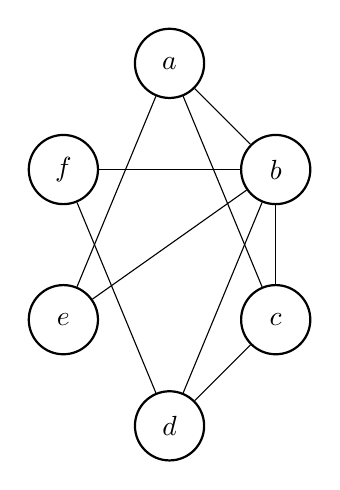
\begin{tikzpicture}
			[-,
			node distance=1cm,
			every state/.style={thick, fill=white!10},
			initial text=$ $,
			]
			\node[state] (a){$a$};
			\node[state, below right =of a] (b){$b$};
			\node[state, below left=of a] (f){$f$};
			\node[state, below =of b] (c) {$c$};
			\node[state, below left=of c] (d) {$d$};
			\node[state, below =of f] (e) {$e$};
			
			\path (e) edge [] node[below] {} (b);
			\path (e) edge [] node[below] {} (a);
			\path (a) edge [] node[below] {} (b);
			\path (c) edge [] node[below] {} (b);
			\path (c) edge [] node[below] {} (a);
			\path (c) edge [] node[below] {} (d);
			\path (b) edge [] node[below] {} (d);
			\path (b) edge [] node[below] {} (f);
			\path (d) edge [] node[below] {} (f);
			
		\end{tikzpicture}
	\end{center}
\end{latin}
از آنجایی که حداقل درجه برای یک راس برابر با ۲ می‌باشد ابتدا تلاش می‌کنیم با ۳ رجیستر این‌ها را پوشش دهیم بنابراین با این فرض جلو می‌رویم،‌ از آنجایی که ۳ رجیستر داریم ابتدا راس f که دارای درجه‌ی دو می‌باشد را حذف می‌کنیم بنابراین گراف به صورت زیر تبدیل می‌شود و صف متغیر‌ها به صورت [f] می‌باشد:
\begin{latin}
	\begin{center}
		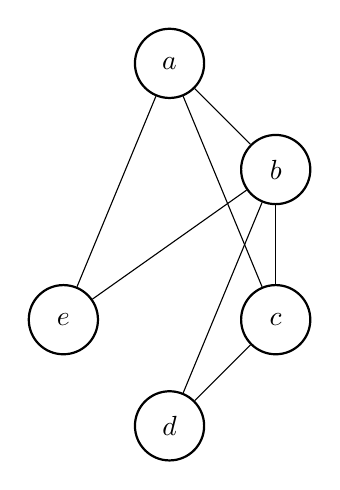
\begin{tikzpicture}
			[-,
			node distance=1cm,
			every state/.style={thick, fill=white!10},
			initial text=$ $,
			]
			\node[state] (a){$a$};
			\node[state, below right =of a] (b){$b$};
			\node[state, below =of b] (c) {$c$};
			\node[state, below left=of c] (d) {$d$};
			\node[state, above left=of d] (e) {$e$};
			
			\path (e) edge [] node[below] {} (b);
			\path (e) edge [] node[below] {} (a);
			\path (a) edge [] node[below] {} (b);
			\path (c) edge [] node[below] {} (b);
			\path (c) edge [] node[below] {} (a);
			\path (c) edge [] node[below] {} (d);
			\path (b) edge [] node[below] {} (d);

			
		\end{tikzpicture}
	\end{center}
\end{latin}
حال با توجه به درجه ۲ بودن e آن را حذف می‌کنیم و صف متغیر‌ها به صورت \lr{[f, e]} و گراف به صورت زیر می‌باشد:
\begin{latin}
	\begin{center}
		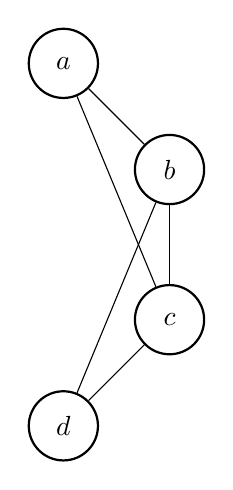
\begin{tikzpicture}
			[-,
			node distance=1cm,
			every state/.style={thick, fill=white!10},
			initial text=$ $,
			]
			\node[state] (a){$a$};
			\node[state, below right =of a] (b){$b$};
			\node[state, below =of b] (c) {$c$};
			\node[state, below left=of c] (d) {$d$};
			
			\path (a) edge [] node[below] {} (b);
			\path (c) edge [] node[below] {} (b);
			\path (c) edge [] node[below] {} (a);
			\path (c) edge [] node[below] {} (d);
			\path (b) edge [] node[below] {} (d);
			
			
		\end{tikzpicture}
	\end{center}
\end{latin}
حال با توجه به درجه ۲ بودن d آن را حذف می‌کنیم و صف متغیر‌ها به صورت  \lr{[f, e, d]} و گراف به صورت زیر می‌باشد:
\begin{latin}
	\begin{center}
		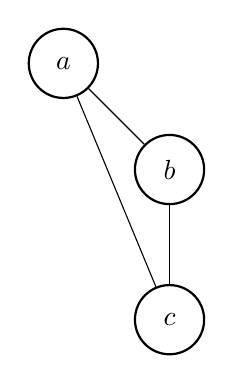
\begin{tikzpicture}
			[-,
			node distance=1cm,
			every state/.style={thick, fill=white!10},
			initial text=$ $,
			]
			\node[state] (a){$a$};
			\node[state, below right =of a] (b){$b$};
			\node[state, below =of b] (c) {$c$};
			
			\path (a) edge [] node[below] {} (b);
			\path (c) edge [] node[below] {} (b);
			\path (c) edge [] node[below] {} (a);
			
			
		\end{tikzpicture}
	\end{center}
\end{latin}
حال با توجه به درجه ۲ بودن c آن را حذف می‌کنیم و صف متغیر‌ها به صورت  \lr{[f, e, d, c]} و گراف به صورت زیر می‌باشد:
\begin{latin}
	\begin{center}
		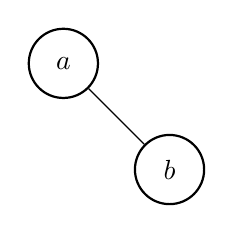
\begin{tikzpicture}
			[-,
			node distance=1cm,
			every state/.style={thick, fill=white!10},
			initial text=$ $,
			]
			\node[state] (a){$a$};
			\node[state, below right =of a] (b){$b$};
			
			\path (a) edge [] node[below] {} (b);
			
			
		\end{tikzpicture}
	\end{center}
\end{latin}
در نهایت نیز متغیر b را از گراف حذف می‌کنیم و پس از آن نیر با حذف a صف به صورت  \lr{[f, e, d, c, b]} می‌باشد حال ابتدا a را رنگ می‌کنیم و در گراف قرار می‌دهیم و گراف به صورت زیر بدست می‌آید:
\begin{latin}
	\begin{center}
		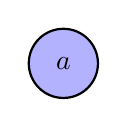
\begin{tikzpicture}
			[-,
			node distance=1cm,
			every state/.style={thick, fill=white!10},
			initial text=$ $,
			]
			\node[state, style={thick, fill=blue!30}] (a){$a$};
			
			
		\end{tikzpicture}
	\end{center}
\end{latin}

حال b را به گراف بر‌می‌گردانیم، صف به صورت \lr{[f, e, d, c]} می‌باشد و در زیر گراف جدید مشاهده می‌شود:
\begin{latin}
	\begin{center}
		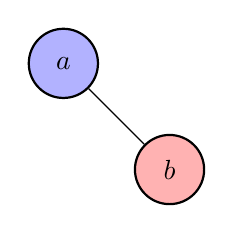
\begin{tikzpicture}
			[-,
			node distance=1cm,
			every state/.style={thick, fill=white!10},
			initial text=$ $,
			]
			\node[state, style={thick, fill=blue!30}] (a){$a$};
			\node[state, style={thick, fill=red!30}, below right =of a] (b){$b$};
			
			\path (a) edge [] node[below] {} (b);
			
		\end{tikzpicture}
	\end{center}
\end{latin}
حال c را به گراف بر می‌گردانیم، صف به صورت \lr{[f, e, d]} می‌باشد و در زیر گراف جدید مشاهده می‌شود:
\begin{latin}
	\begin{center}
		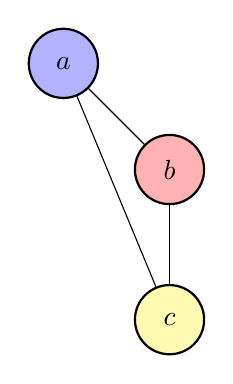
\begin{tikzpicture}
			[-,
			node distance=1cm,
			every state/.style={thick, fill=white!10},
			initial text=$ $,
			]
			\node[state, style={thick, fill=blue!30}] (a){$a$};
			\node[state, style={thick, fill=red!30}, below right =of a] (b){$b$};
			\node[state, style={thick, fill=yellow!30}, below =of b] (c) {$c$};
			\path (a) edge [] node[below] {} (b);
			\path (c) edge [] node[below] {} (b);
			\path (c) edge [] node[below] {} (a);
			
		\end{tikzpicture}
	\end{center}
\end{latin}

حال d را به گراف بر می‌گردانیم، صف به صورت \lr{[f, e]} می‌باشد و در زیر گراف جدید مشاهده می‌شود:
\begin{latin}
	\begin{center}
		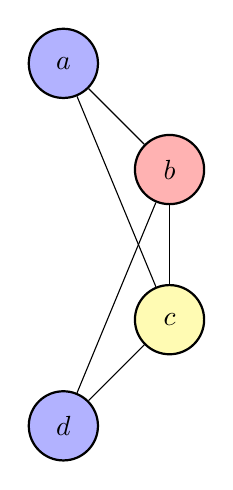
\begin{tikzpicture}
			[-,
			node distance=1cm,
			every state/.style={thick, fill=white!10},
			initial text=$ $,
			]
			\node[state, style={thick, fill=blue!30}] (a){$a$};
			\node[state, style={thick, fill=red!30}, below right =of a] (b){$b$};
			\node[state, style={thick, fill=yellow!30}, below =of b] (c) {$c$};
			\node[state, style={thick, fill=blue!30}, below left=of c] (d) {$d$};
			
			\path (a) edge [] node[below] {} (b);
			\path (c) edge [] node[below] {} (b);
			\path (c) edge [] node[below] {} (a);
			\path (c) edge [] node[below] {} (d);
			\path (b) edge [] node[below] {} (d);
			
		\end{tikzpicture}
	\end{center}
\end{latin}

حال e را به گراف بر می‌گردانیم، صف به صورت \lr{[f]} می‌باشد و در زیر گراف جدید مشاهده می‌شود:
\begin{latin}
	\begin{center}
		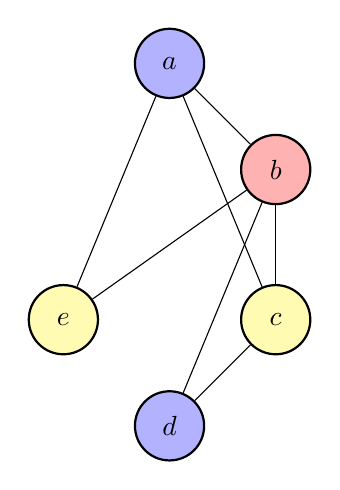
\begin{tikzpicture}
			[-,
			node distance=1cm,
			every state/.style={thick, fill=white!10},
			initial text=$ $,
			]
			\node[state, style={thick, fill=blue!30}] (a){$a$};
			\node[state, style={thick, fill=red!30}, below right =of a] (b){$b$};
			\node[state, style={thick, fill=yellow!30}, below =of b] (c) {$c$};
			\node[state, style={thick, fill=blue!30}, below left=of c] (d) {$d$};
			\node[state, style={thick, fill=yellow!30}, above left=of d] (e) {$e$};
			
			\path (e) edge [] node[below] {} (b);
			\path (e) edge [] node[below] {} (a);
			\path (a) edge [] node[below] {} (b);
			\path (c) edge [] node[below] {} (b);
			\path (c) edge [] node[below] {} (a);
			\path (c) edge [] node[below] {} (d);
			\path (b) edge [] node[below] {} (d);
			
		\end{tikzpicture}
	\end{center}
\end{latin}



حال f را به گراف بر می‌گردانیم با توجه به اینکه b,d راس‌های مجاور آن می‌باشند رنگ f برابر با زرد می‌شود:
\begin{latin}
	\begin{center}
		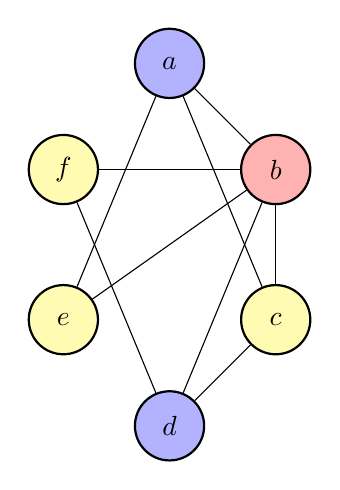
\begin{tikzpicture}
			[-,
			node distance=1cm,
			every state/.style={thick, fill=white!10},
			initial text=$ $,
			]
			\node[state, style={thick, fill=blue!30}] (a){$a$};
			\node[state, style={thick, fill=red!30}, below right =of a] (b){$b$};
			\node[state, style={thick, fill=yellow!30}, below =of b] (c) {$c$};
			\node[state, style={thick, fill=blue!30}, below left=of c] (d) {$d$};
			\node[state, style={thick, fill=yellow!30}, above left=of d] (e) {$e$};
			\node[state, style={thick, fill=yellow!30}, above=of e] (f) {$f$};
			
			\path (e) edge [] node[below] {} (b);
			\path (e) edge [] node[below] {} (a);
			\path (a) edge [] node[below] {} (b);
			\path (c) edge [] node[below] {} (b);
			\path (c) edge [] node[below] {} (a);
			\path (c) edge [] node[below] {} (d);
			\path (b) edge [] node[below] {} (d);
			\path (b) edge [] node[below] {} (f);
			\path (d) edge [] node[below] {} (f);
			
		\end{tikzpicture}
	\end{center}
\end{latin}




%نام و نام خانوادگی:
%شماره دانشجویی: 
\مسئله{پارسر \lr{LALR(1)}}

\پاسخ{ }
\\
الف) عکس دیاگرام در زیر قرار داده شده است:
\graphicspath{{./images/}}
\begin{center}
	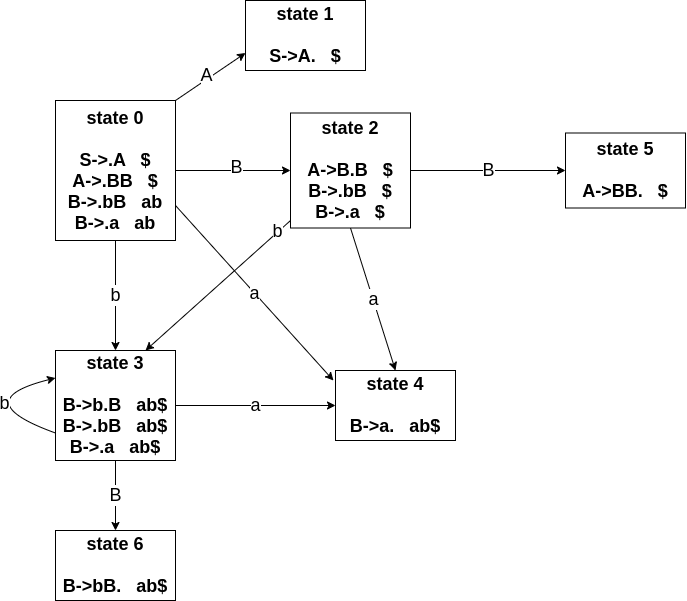
\includegraphics[scale=0.7]{compiler_hw2_q9.png}
\end{center}
عکس جدول در زیر قرار داده شده است:
\include{{./images}}
\begin{center}
	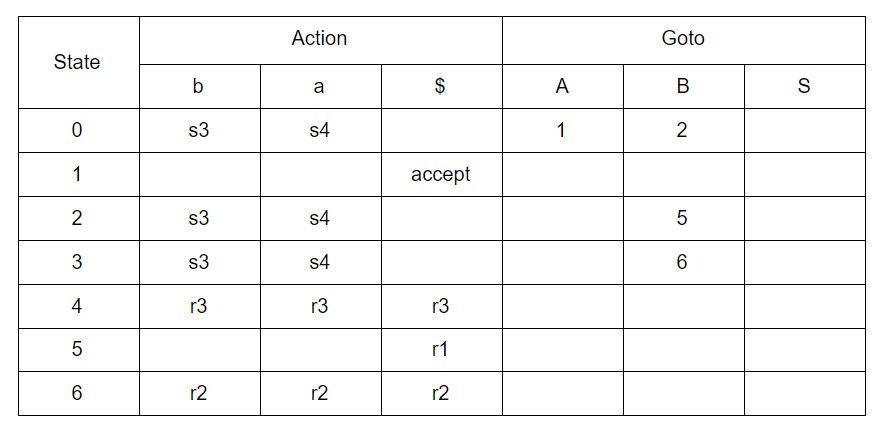
\includegraphics[scale=0.9]{compiler_hw2_q9_table.png}
\end{center}
ب) درخت پارس $babba$ را در پایین نوشته‌ایم: (دقت شود که حروفی که بین دو | می‌آیند در مرحله بعدی قرار است با هم، به کمک قاعده تولید reduce شوند)
\begin{latin}
	b
	\\
	b a
	\\
	b |a|
	\\
	b B
	\\
	|b B|
	\\
	B
	\\
	B b
	\\
	B b b
	\\
	B b b a
	\\
	B b b |a|
	\\
	B b b B
	\\
	B b |b B|
	\\
	B b B
	\\
	B |b B|
	\\
	B B
	\\
	|B B|
	\\
	A
\end{latin}
در نهایت درخت پارس رشته به صورت زیر می‌شود:
\begin{center}
	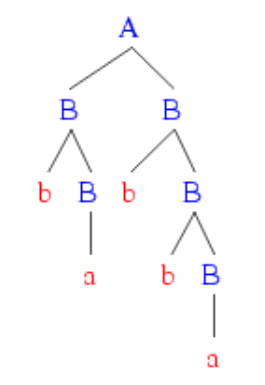
\includegraphics{babba.png}
\end{center}












%نام و نام خانوادگی:
%شماره دانشجویی: 
\مسئله{مقایسه‌ی \lr{LR(1)} و \lr{SLR(1)}}

\پاسخ{ }
   
\end{document}

